\documentclass[10pt]{beamer}

%%%
% PREAMBLE FOR THIS DOC 
%%%
%https://tex.stackexchange.com/questions/68821/is-it-possible-to-create-a-latex-preamble-header
\usepackage{/Users/miw267/Repos/csci246_fall2025/slides/preambles/beamer_preamble_for_CSCI246}



%%% TRY TO RESHOW TOC AT EACH SECTION START (with current section highlighted)
% Reference: https://tex.stackexchange.com/questions/280436/how-to-highlight-a-specific-section-in-beamer-toc
\newcommand\tocforsect[2]{%
  \begingroup
  \edef\safesection{\thesection}
  \setcounter{section}{#1}
  \tableofcontents[#2,currentsection]
  \setcounter{section}{\safesection}
  \endgroup
}


%%%% HERES HOW TO DO IT CORRECTLY
% FIRST IN .STY FILE, DO
%\usetheme[sectionpage=none]{metropolis}
% THEN AT EACH SECTION DO
%\begin{frame}{Outline}
%  \tableofcontents[currentsection]	
%\end{frame}



%\setbeamertemplate{navigation symbols}{}
%\setbeamertemplate{footline}[frame number]{}

%%% SPECIAL FOR THIS DOC
\usetikzlibrary{arrows.meta}

%%%
% DOCUMENT
%%%

\begin{document}

%\maketitle

%% Title page frame
%\begin{frame}
%    \titlepage 
%\end{frame}




\title{09/23/2026: Relations}
\author{CSCI 246: Discrete Structures}
\date{Textbook reference: Sec 14, Scheinerman}

\begin{frame}
    \titlepage 
\end{frame}


\begin{frame}
\footnotesize 

%\begin{myredbox}[title=Announcements]
%
%\begin{itemize}
%\item Please remember to write your last name on the back of your quiz.
%\end{itemize}
%
%\end{myredbox}
%\vfill 


\begin{myyellowbox}[title=Today's Agenda]
\begin{itemize}
	\item Review group exercises ($\approx$ 10 mins)
	\item Mini-lecture ($\approx$ 20 mins)
	\item Group exercises ($\approx$ 15 mins)
\end{itemize}


%	
\end{myyellowbox}
\vfill 

\end{frame}


\begin{frame}{Study Guide For Quiz 4}
\footnotesize 


\colorbox{red!20}{\textbf{Readings.}} 
Sec. 10 (Sets)
\begin{itemize}
\item Know how to apply the strategy for proving that two sets are equal (Proof Template 5). In particular, know how to prove Prop 10.1.
\item Know how to count the number of subsets of a set.
\end{itemize}
Sec. 11 (Quantifiers)
\begin{itemize}
\item Know how to apply the strategy for proving existential statements (Proof Template 7) to Example 11.1. Know how to apply the strategy for proving universal statements (Proof Template 8) to Example 11.2.
\item Know how to read and negate quantified statements.
\end{itemize}
Sec. 12 (Set Operations)
\begin{itemize}
\item From Theorem 12.3, know how to prove the associative properties (see text) and distributive properties (see slides).
\item Know how to apply Prop 12.4 (the size of a union) to solve Example 12.5.
\item Know how to prove Prop 12.11 (alternative form of symmetric difference).
\end{itemize}


\vfill 
\colorbox{yellow!20}{\textbf{Group exercises.}} Know how to do all of the group exercises from the course meetings on Sets (9/16), Quantifiers (9/18), and Set Operations (9/21).


\end{frame}

%\begin{frame}
%
%\small
% \begin{myredbox}[title=\text{Weekly Quiz \#4}] 
%\begin{enumerate}
%	\item \textit{(Sec. 10 -- Sets.)} Prove that the following two sets are equal	:
%	%
%	\begin{align*}
%	E &= \set{x \in \mathbb{Z} : x \text{ is even}}, \qquad \text{and} \\
%	F &= \set{z \in \mathbb{Z} : z = a+b \text{ where $a$ and $b$ are both odd}}.	
%	\end{align*}
%	
%	\item \textit{(Sec. 11 -- Quantifiers.)}   For each sentence below, write the negation of the sentence in quantified form. Then rewrite the negation in English.  
%    \begin{itemize}
%    
%        \item[a.] $\forall x \in \mathbb{Z}, x \text{ is odd.} $ 
%        \item[b.] $\exists x \in \mathbb{Z}: \forall y \in \mathbb{Z}, x>y.$
%        \item[c.]  $\forall x \in \mathbb{Z}, \forall y \in \mathbb{Z}, x=y.$
%    \end{itemize}
%
%	\item \textit{(Sec. 12 -- Set Operations.)}  Prove the second distributive property below.
%	\[ A \cup (B \cap C) = (A \cup B) \cap (A \cup C), \quad \text{and} \quad  A \cap (B \cup C) = (A \cap B) \cup (A \cap C). \]
%\end{enumerate}
%\end{myredbox}
%\vfill 
%\begin{mygreenbox}[title=\text{Reference Material: Distributive Properties of Boolean Algebra}]
%	\[ x \land (y \lor z) = (x \land y) \lor (x \land z), \quad \text{and} \quad  x \lor (y \land z) = (x \lor y) \land (x \lor z). \]
%\end{mygreenbox}
%
%\end{frame}


%%%% Section
\begin{frame}[standout]
Outline for Mini-Lecture:
\begin{itemize}
\item \alert{\textbullet \quad Introduction}
\item \textbullet \quad Drawing relations as pictures 
\item \textbullet \quad Properties of relations 
\item \textbullet \quad Drawing properties as pictures
\item \textbullet \quad Applications
\end{itemize}
\end{frame}




\begin{frame}{Relations}
\small 
A \textbf{relation} is just a set of ordered pairs that connect elements of one set to another (or the same set).
\vfill 
\pause 

\begin{mybluebox}[title=Example]
\begin{itemize}
\item Let $P$ be a set of people. Let $C$ be a set of cities.	
\item Define the relation $R \subseteq P \times C$ by 
\[ R = \set{(p,c) : \text{ person $p$ has lived in city $c$.}} \] 
\end{itemize}


\begin{center}
\resizebox{0.5\textwidth}{!}{%
\begin{tikzpicture}[>={Stealth[length=8pt,width=6pt]}, node distance=3mm, thick]

  % People nodes
  \node (Mike) {\Large Mike};
  \node[below=of Mike] (Paul) {\Large Paul};
  % Ellipse around P
  \node[draw, ellipse, fit=(Mike)(Paul), inner sep=1mm] (P) {};
  \node at (P.north) [above] {\Large $P$};

  % City nodes
  \node[right=5cm of Mike] (Bozeman) {\Large Bozeman};
  \node[above=of Bozeman] (Jacksonville) {\Large Jacksonville, FL};
  \node[above=of Jacksonville] (Seattle) {\Large Seattle};
  \node[below=of Bozeman] (Rockfield) {\Large Rockfield, MD};
  \node[below=of Rockfield] (Butte) {\Large Butte};
  \node[below=of Butte] (Billings) {\Large Billings};
  % Ellipse around C
  \node[draw, ellipse, fit=(Bozeman)(Jacksonville)(Seattle)(Rockfield)(Butte)(Billings),
        inner sep=1mm] (C) {};
  \node at (C.north) [above] {\Large $C$};

  % Arrows from Mike
  \draw[->] (Mike.east) -- (Bozeman.west);
  \draw[->] (Mike.east) -- (Seattle.west);
  \draw[->] (Mike.east) -- (Jacksonville.west);

  % Arrows from Megan
  \draw[->] (Paul.east) -- (Bozeman.west);
  \draw[->] (Paul.east) -- (Rockfield.west);
  \draw[->] (Paul.east) -- (Butte.west);

\end{tikzpicture}
}
\end{center}
\end{mybluebox}
\end{frame}

\begin{frame}
\footnotesize


\begin{mybluebox}[title=Example]
Let $A = \set{2,3,4,5,6}$ and $B=\set{3,6,9}$ and relation $R=\set{(a,b): a|b, a \in A, b \in B}$.  Then  $R=$ \only<2->{$\set{(2,6), (3,3), (3,6), (3,9), (6,6)}$.} 

\only<3->{
\begin{figure}
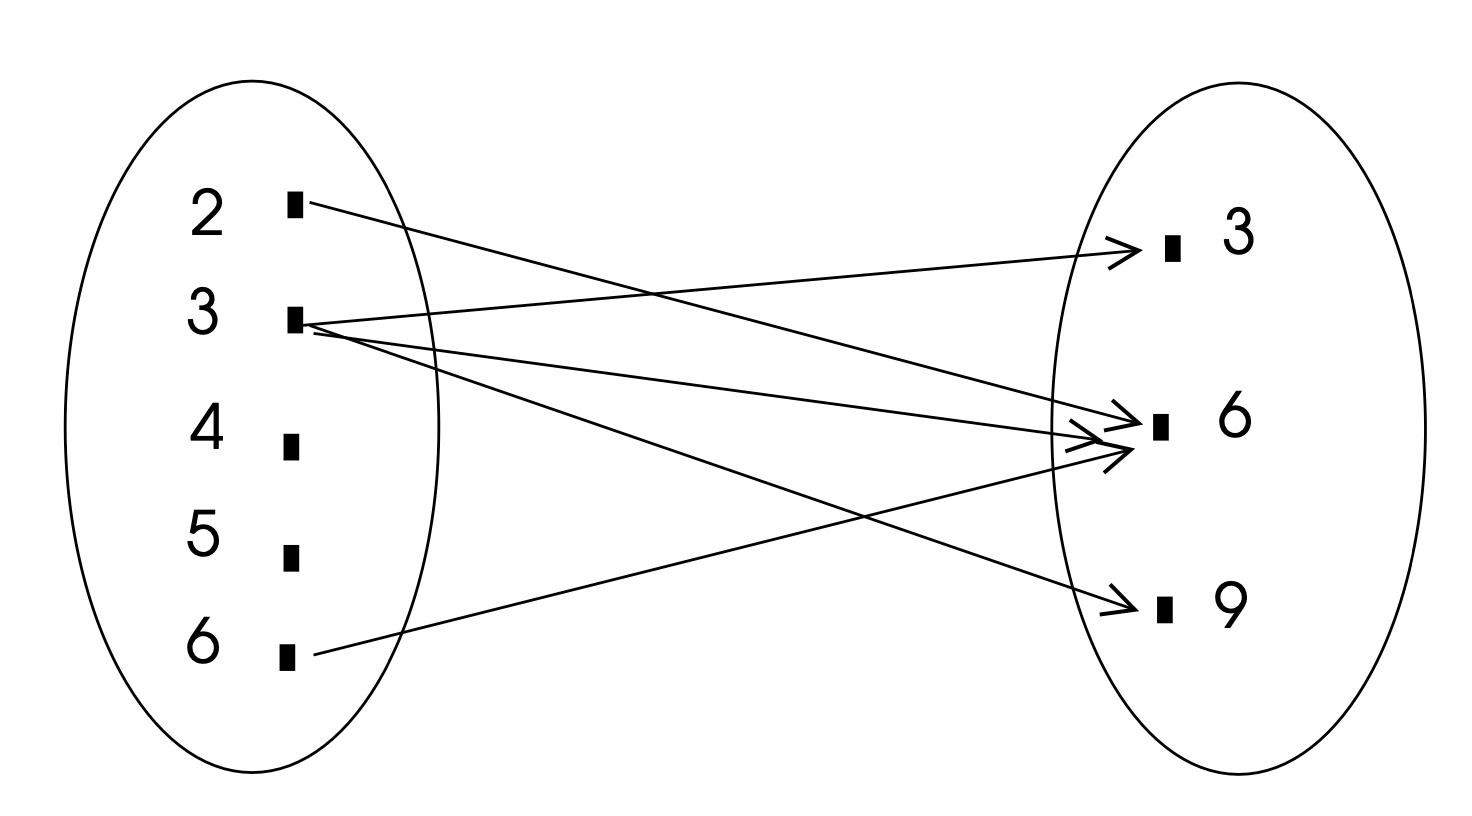
\includegraphics[width=.5\textwidth]{images/relation_example.png}	
\caption{Set diagram representation of the relation $R$}
\end{figure}
}

\end{mybluebox}

\vfill 


\only<4->{
\begin{mygreenbox}[title=Definition (Hampkins)]
Let $A$ and $B$ be two sets.  A \textbf{binary relation} (or simply a \textbf{relation}) $R$ from $A$ to $B$ is a subset of the Cartesian product $A \times B$.
\end{mygreenbox}
}


\vfill 

 
\only<5->{ 
\begin{mygreenbox}[title=Definition (Scheinerman Def 14.1)]
A \textbf{relation} is a set of ordered pairs.
\end{mygreenbox}
}	
\end{frame}

\begin{frame}{Relations: Some odds and ends}

\begin{myredbox}[title=Notation]
If $(a,b) \in R$, we write $aRb$.	
\end{myredbox}

\vfill 
\pause 


\colorbox{green!30}{\textbf{Example.}}
\begin{itemize}
	\item Let $A=B=\mathbb{Z}$, and $R=$\qq{$\leq$}.
	\item Then $2R2$ and $2R3$ but $3 \cancel{R} 2$.
\end{itemize}
\vfill 
\pause 
\colorbox{red!30}{\textbf{Warning.}} \warning As the above shows, relations in math are \alert{uni-directional}.
\vfill 
\pause 
\colorbox{yellow!30}{\textbf{Poll.}} How is a relation different from a function?
\vfill 
\pause 
\colorbox{green!30}{\textbf{Solution.}} An $a \in A$ can connect to \alert{more than one} $b \in B$.   For example:
\vspace{-0.5cm}
\begin{itemize}
\item Let $R$ be the relation \texttt{has-lived-in-city}.
\item Let $m = \texttt{Mike}, b=\texttt{Bozeman}, s=\texttt{Seattle}$.
\item Then we have $mRb$ \alert{and} $mRs$.	
\end{itemize}

\vfill 
\pause 




\end{frame}

%%%% Section
\begin{frame}[standout]
Outline for Mini-Lecture:
\begin{itemize}
\item \textbullet \quad Introduction
\item \alert{\textbullet \quad Drawing relations as pictures} 
\item \textbullet \quad Properties of relations 
\item \textbullet \quad Drawing properties as pictures
\item \textbullet \quad Applications
\end{itemize}
\end{frame}


\begin{frame}

\begin{myredbox}[title=Drawing relations from $A$ to $B$]
To depict a relation $R$ from $A$ to $B$, place dots for $A$ on the left and for $B$ on the right, then draw an arrow from $a \in A$ to $b \in B$ whenever $(a,b) \in R$.
 \end{myredbox}
 
\begin{mygreenbox}[title=Example]
\begin{itemize}
\item 	Let $A = \set{1,2,3,4,5}$ and $B=\set{4,5,6,7}$.
\item Let $R$ be the relation $\set{(1,4),(1,5),(2,5),(3,6)}$.
\item Then the figure below shows $R$ as a picture.
\end{itemize} 
 
 \begin{figure}
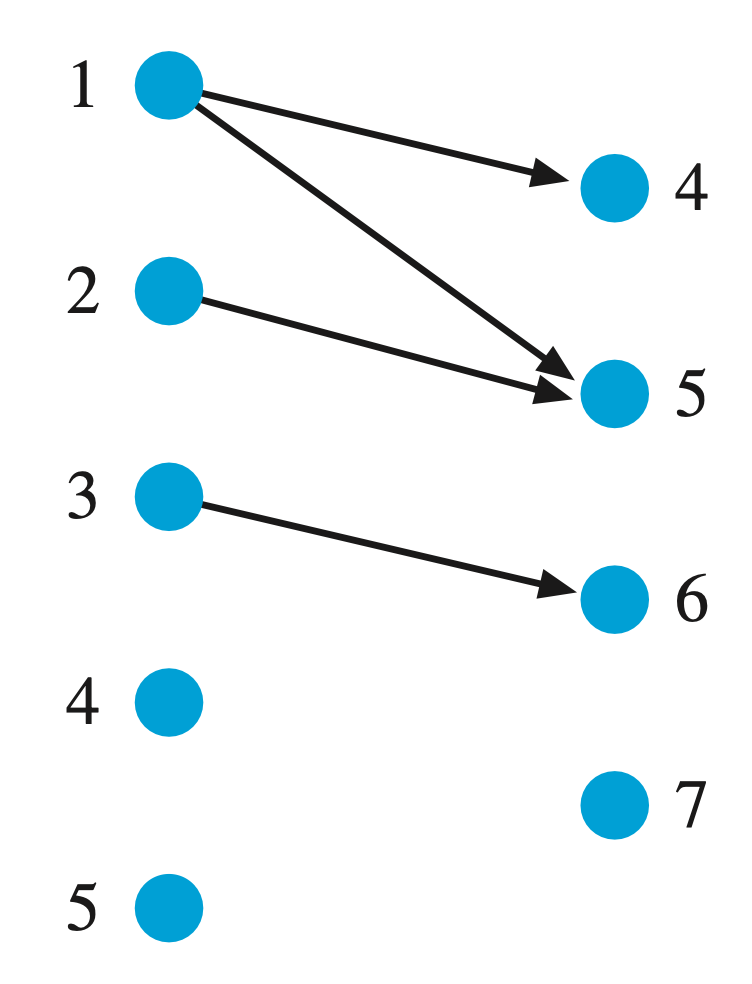
\includegraphics[width=.3\textwidth]{images/relations} 
\end{figure}

\end{mygreenbox}
 


\end{frame}


\begin{frame}

\begin{myredbox}[title=Drawing relations on $A$]
To draw a relation $R$ on $A$, either:
\begin{enumerate}
	\item View $R$ as a relation from $A$ to itself and use the previous method.
	\item Represent each element of $A$ as a dot and draw arrows for pairs $(a,b)\in R$ (including loops if $aRa$).
\end{enumerate}
 \end{myredbox}
 
\begin{mygreenbox}[title=Example]
\begin{itemize}
\item 	Let $A = \set{1,2,3,4,5}$.
\item Let $R=\set{(1,1), (1,2), (1,3), (4,3), (3,1)}$.
\item  A picture of the relation $R$ (using option \#2) is given below.  
\end{itemize} 
 
 \begin{figure}
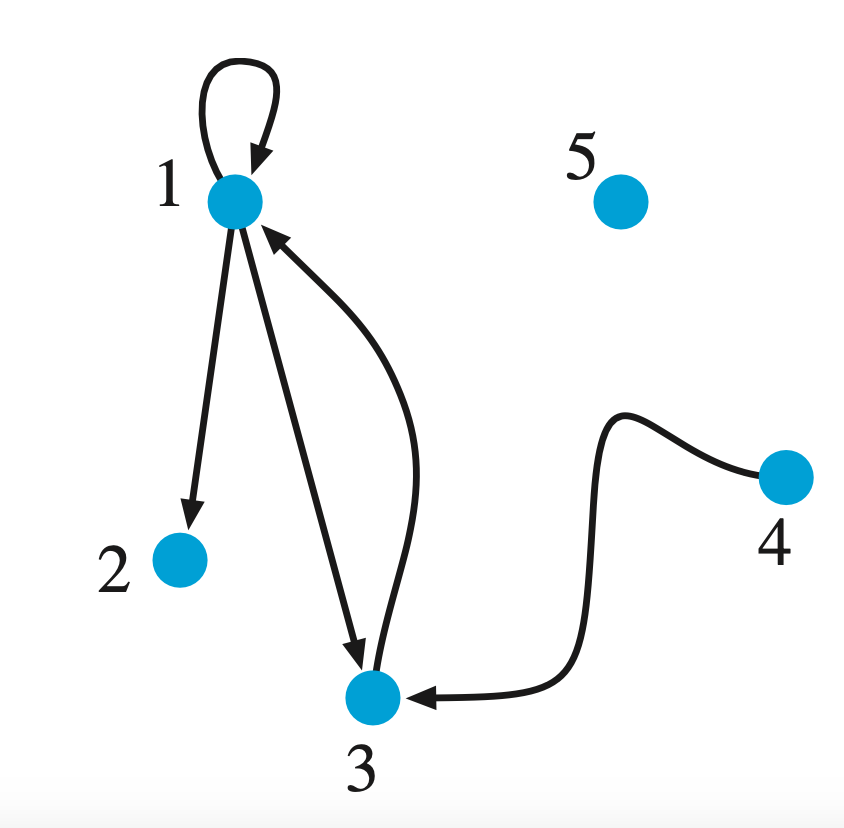
\includegraphics[width=.3\textwidth]{images/relations_on_A} 
\end{figure}

\end{mygreenbox}
 


\end{frame}



\begin{frame}

\begin{mygreenbox}[title=An Example Using a Set with Infinitely Many Elements]
Let $A = \mathbb{Z}$ and $R$ be the $\leq$ relation.  A picture of the relation is given below 
 \begin{figure}
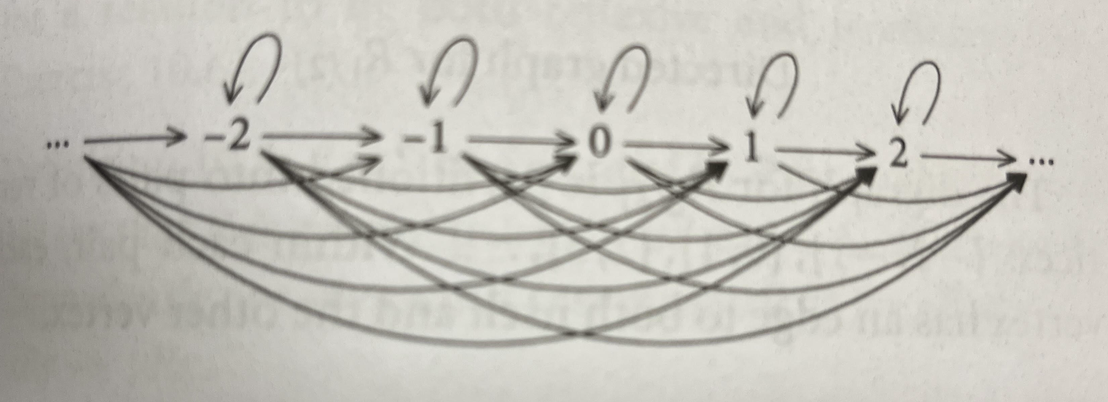
\includegraphics[width=\textwidth]{images/leq} 
\end{figure}

\end{mygreenbox}
 \end{frame}
 


%%%% Section
\begin{frame}[standout]
Outline for Mini-Lecture:
\begin{itemize}
\item \textbullet \quad Introduction
\item \textbullet \quad Drawing relations as pictures
\item \alert{\textbullet \quad Properties of relations} 
\item \textbullet \quad Drawing properties as pictures
\item \textbullet \quad Applications
\end{itemize}
\end{frame}



\begin{frame}
 
\small 
 \begin{mygreenbox}[title=Definition]
Suppose that $R$ is a relation on a set $A$.
\begin{enumerate}
	\item The relation $R$ is \textbf{reflexive} on $A$ if $a\,R\,a$ for all $a \in A$.
	\item  The relation $R$ is \textbf{symmetric} on $A$ if, whenever $a\,R\,b$, then also $b\,R\,a$.
	\item The relation $R$ is \textbf{transitive} on $A$ if, whenever $a\,R\,b$ and $b\,R\,c$, then also $a\,R\,c$.
\end{enumerate}
\end{mygreenbox}
\vfill 
\colorbox{yellow!30}{\textbf{Poll.}} Let $A$ be the set of people. Can you think of an example and counterexample for each property?
\vfill 
\pause 
\begin{mybluebox}[title=Examples]
Let $A$ be the set of people.
\begin{enumerate}
	\item \textbf{Reflexivity.} \pause The \texttt{lives-in-the-same-city-as} relation is reflexive, but the \texttt{parent-of} relation is not. 
	\vspace{-.2cm} 
	\item \textbf{Symmetry.} \pause The \texttt{friends-of} relation is symmetric (usually -- 
\includegraphics[height=1em]{images/eek}), but \texttt{parents-of} relation is not. 
	\item \textbf{Transitivity.} \pause The \texttt{is-in-the-same-family} relation is transitive, but the \texttt{parent-of} relation is not. 
\end{enumerate}
	
\end{mybluebox}

\end{frame}



%%%% Section
\begin{frame}[standout]
Outline for Mini-Lecture:
\begin{itemize}
\item \textbullet \quad Introduction
\item \textbullet \quad Drawing relations as pictures
\item \textbullet \quad Properties of relations
\item \alert{\textbullet \quad Drawing properties as pictures}
\item \textbullet \quad Applications
\end{itemize}
\end{frame}


\begin{frame}
\footnotesize 

\begin{myyellowbox}[title=Reflexivity]
\begin{itemize}
	\item A relation is \textbf{reflexive} if every element has a self-loop.  \pause 
	\item A relation is \textbf{not reflexive} if\only<2>{\alert{\textbf{ what?}}}\only<3->{ at least one element has no self-loop.}
\end{itemize}
\end{myyellowbox}

\vfill 
\only<4>{
\begin{mygreenbox}[title=Example]
\begin{table}[H]
\centering 	
\begin{tabular}{cc}
\textbf{Reflexive} & \textbf{Not reflexive}  \\
$\forall \; x \in A,  xRx$	& $\exists \; x \in A :  x\cancel{R}x$\\
\begin{tikzpicture}

% Nodes in a vertical line
\node[latent] (1) at (0, 4) {a};
\node[latent] (2) at (0, 3) {b};
\node[latent] (3) at (0, 2) {c};
\node[latent] (4) at (0, 1) {d};


% Self loops
\path[->, >=stealth, loop left, red] (1) edge (1);
\path[->, >=stealth, loop left, red] (2) edge (2);
\path[->, >=stealth, loop left, red] (3) edge (3);
\path[->, >=stealth, loop left, red] (4) edge (4);

% Curved edges
\path[->, >=stealth, bend left=60] (1) edge (2);
\path[->, >=stealth, bend left=60] (1) edge (4);
\path[->, >=stealth, bend left=60] (2) edge (4);
\end{tikzpicture} 
& 
\begin{tikzpicture}

% Nodes in a vertical line
\node[latent] (1) at (0, 4) {a};
\node[latent] (2) at (0, 3) {b};
\node[latent] (3) at (0, 2) {c};
\node[latent] (4) at (0, 1) {d};

% Curved edges
\path[->, >=stealth, bend left=60] (1) edge (2);
\path[->, >=stealth, bend left=60] (1) edge (4);
\path[->, >=stealth, bend left=60] (2) edge (4);

% Self loops
\path[->, >=stealth, loop left, red] (1) edge (1);
\path[->, >=stealth, loop left, red] (3) edge (3);
\end{tikzpicture} 

\end{tabular}
\end{table}

When one or more red connection drops out, the relation loses reflexivity.
\end{mygreenbox}
}

\end{frame}


\begin{frame}
\footnotesize 

\begin{myyellowbox}[title=Symmetric]
\begin{itemize}
	\item A relation is \textbf{symmetric} if every connection to a distinct element is paired with a connection in the opposite direction.   \pause 
	\item A relation is \textbf{not symmetric} if\only<2>{\alert{ what?}}\only<3->{ at least one connection to a distinct element lacks a connection in the opposite direction.}
\end{itemize}

\end{myyellowbox}

\vfill 
\only<4->{
\begin{mygreenbox}[title=Example]
\begin{table}[H]
\centering 	
\begin{tabular}{cc}
\textbf{Symmetric} & \textbf{Not symmetric}  \\
$xRy \implies yRx$	& $\exists \; x,y \in A :  xRy$ but  $y\cancel{R}x$\\
\begin{tikzpicture}

% Nodes in a vertical line
\node[latent] (1) at (0, 4) {a};
\node[latent] (2) at (0, 3) {b};
\node[latent] (3) at (0, 2) {c};
\node[latent] (4) at (0, 1) {d};


% Self loops
\path[->, >=stealth, loop left] (1) edge (1);
\path[->, >=stealth, loop left] (3) edge (3);

% Curved edges
\path[->, >=stealth, bend left=60] (1) edge (2);
\path[->, >=stealth, bend left=60] (2) edge (1);
\path[->, >=stealth, bend left=60] (2) edge (3);
\path[->, >=stealth, bend left=60] (3) edge (2);
\path[->, >=stealth, bend left=60] (1) edge (4);
\path[->, >=stealth, bend left=60] (4) edge (1);
\end{tikzpicture} 
& 
\begin{tikzpicture}

% Nodes in a vertical line
\node[latent] (1) at (0, 4) {a};
\node[latent] (2) at (0, 3) {b};
\node[latent] (3) at (0, 2) {c};
\node[latent] (4) at (0, 1) {d};

% Curved edges
\path[->, >=stealth, bend left=60] (1) edge (2);
\path[->, >=stealth, bend left=60] (2) edge (1);
\path[->, >=stealth, bend left=60] (2) edge (3);
\path[->, >=stealth, bend left=60] (3) edge (2);
\path[->, >=stealth, bend left=60] (1) edge (4);
%\path[->, >=stealth, bend left=60] (4) edge (1);


% Self loops
\path[->, >=stealth, loop left] (1) edge (1);
\path[->, >=stealth, loop left] (3) edge (3);
\end{tikzpicture} 

\end{tabular}
\end{table}

When we dropped the connection from $d$ to $a$, the relationship lost symmetry.

\end{mygreenbox}
}

\end{frame}


\begin{frame}
\footnotesize 

\begin{myyellowbox}[title=Transitivity]
\begin{itemize}
	\item A relation is \textbf{transitive} if every two-hop trip can also be done in a single-hop.  \pause 
	\item A relation is \textbf{not transitive} if \only<2>{\alert{what?}}\only<3->{there is at least one two-hop trip that cannot be done in a single hop.}
\end{itemize}

\end{myyellowbox}

\vfill 
\only<4->{
\begin{mygreenbox}[title=Example]
\begin{table}[H]
\centering 	
\begin{tabular}{cc}
\textbf{Transitive} & \textbf{Not transitive}  \\
$xRy, yRz \implies xRz$	& $\exists \; x,y,z \in A :  xRy$ and $yRz$ but  $x\cancel{R}z$\\
\begin{tikzpicture}

% Nodes in a vertical line
\node[latent] (1) at (0, 4) {a};
\node[latent] (2) at (0, 3) {b};
\node[latent] (3) at (0, 2) {c};
\node[latent] (4) at (0, 1) {d};


% Self loops
\path[->, >=stealth, loop left] (4) edge (4);

% Curved edges
\path[->, >=stealth, bend left=60] (1) edge (2);
\path[->, >=stealth, bend left=60] (2) edge (3);
\path[->, >=stealth, bend left=60] (1) edge (3);
\end{tikzpicture} 
& 
\begin{tikzpicture}

% Nodes in a vertical line
\node[latent] (1) at (0, 4) {a};
\node[latent] (2) at (0, 3) {b};
\node[latent] (3) at (0, 2) {c};
\node[latent] (4) at (0, 1) {d};

% Self loops
\path[->, >=stealth, loop left] (4) edge (4);

% Curved edges
\path[->, >=stealth, bend left=60] (1) edge (2);
\path[->, >=stealth, bend left=60] (2) edge (3);
%\path[->, >=stealth, bend left=60] (1) edge (3);

\end{tikzpicture} 

\end{tabular}
\end{table}

When we dropped the connection from $a$ to $c$, the relationship lost transitivity.

\end{mygreenbox}
}

\end{frame}



%%%% Section
\begin{frame}[standout]
Outline for Mini-Lecture:
\begin{itemize}
\item \textbullet \quad Introduction
\item \textbullet \quad Drawing relations as pictures
\item \textbullet \quad Properties of relations
\item \textbullet \quad Drawing properties as pictures
\item \alert{\textbullet \quad Applications}
\end{itemize}
\end{frame}




\begin{frame}{Example of Relations in Computer Science}
\footnotesize 
\begin{mygreenbox}[title=Example]

Let's consider a ``friendship" relation in a \textbf{social network} like Facebook. We can define a relation $R$ on a set of users where: $(x,y) \in R$ if and only if $x$ is a friend of $y$. 
\end{mygreenbox}

\begin{myyellowbox}[title=Poll]
Is this relation
\begin{itemize}
\item Reflexive? \pause \redx Users don't usually friend themselves in social networks. 
\item Symmetric? \pause \greencheck(-ish.) In most social networks, a friendship connection is bidirectional. If Alice is a friend of Bob, then Bob is a friend of Alice.  However, in platforms like X (formerly Twitter), where following is \textit{one-way}, the "follows" relation is \textit{not symmetric}.
\item Transitive? \pause \redx If  Alice is friends with Bob and Bob is friends with Charlie, it does not necessarily mean that Alice is friends with Charlie.  %However, in certain recommendation systems, the transitive property may be used to suggest friends-of-friends.
\end{itemize}
\end{myyellowbox}
	
\end{frame}


\begin{frame}

\begin{mygreenbox}[title=Why do relations matter?: Some examples from social networks]

\begin{itemize}
\item \textbf{Social Influence \& Virality}

\begin{itemize}
\item If relationships in a network are \alert{transitive}, messages, trends, and viral content can spread faster.
\end{itemize}

\item \textbf{Friend-of-a-Friend Recommendations}  
\begin{itemize}
\item Even if friendship is not strictly \alert{transitive}, many recommendation algorithms use approximate transitivity to suggest new friends (e.g., LinkedIn’s "People You May Know" feature).
\end{itemize}


\item \textbf{Algorithm Optimization}
\begin{itemize}
\item If a relation is \alert{symmetric}, storage can be optimized by only storing one direction of the connection.
\item Search algorithms (e.g., shortest path) can be optimized by reducing redundant checks.
\end{itemize}
\end{itemize}
\end{mygreenbox}

\end{frame}


\end{document}
